%\section{Adiabatic approximation}
%\label{sec:dis}
%\subsection{Adiabatic invariant}
%the adiabatic invariant 
For the resonant electrons trapped by the slowly varying wave envelope and circling around in the phase space,  the adiabatic invariant is defined as
%at a given $s_i$,
\begin{equation}\label{eq.def_I}
    \mathcal{I} = \frac{1}{2\pi} \oint \Omega(H,\xi,t) \mathrm{d} \xi~,
\end{equation}
where $\Omega$ is an implicit function of the Hamiltonian $H$.
%From the above-mentioned
Using the Hamiltonian (\ref{eq.H_lab}) and (\ref{eq.H_frame}), 
%combining the equation of the moving frame along magnetic field line, 
we can numerically calculate the adiabatic invariant $\mathcal{I}$  in the static and moving resonance frames, respectively.

%verify I is invariant
%for different alpha, if the particle remain trapped...
%To do so, we first iterate the phase space flow with time step $\Delta T$ for one fixed $K_i$ at a given $s_i$ and the corresponding background parameters. 
%Then we push the particle to the next location along the field line. 
%For the deeply trapped particle, we just push the particle to the adjacent cell, which is competitive with our Vlasov simulation.
%At new location, we again trace the phase flow with updated background parameter, wave field and new $K_i$.
%By iteratively following the field lines and tracing in phase space, we can construct a continuous trajectory for a particle.

For each temporospatial location, with fixed background and wave parameters, we are able to complete a closed trajectory if the particle stay trapped in the wave field.  
The area of the enclosed loop is actually the phase space integral $\mathcal{I}$.
%Here, , to illustrate the adiabatic invariant, we calculate the closed phase trajectories with parameter at the initial and at the $s=540$, $t=910$ location.
In the static frame, it is clear that the area changes significantly,
as shown in Fig. \ref{fig.traj}(c). In the moving frame, the area changes much smaller, suggesting the validity of the particle adiabatic motion, as shown in Fig. \ref{fig.traj}(d). 

\begin{figure}
    \centering
    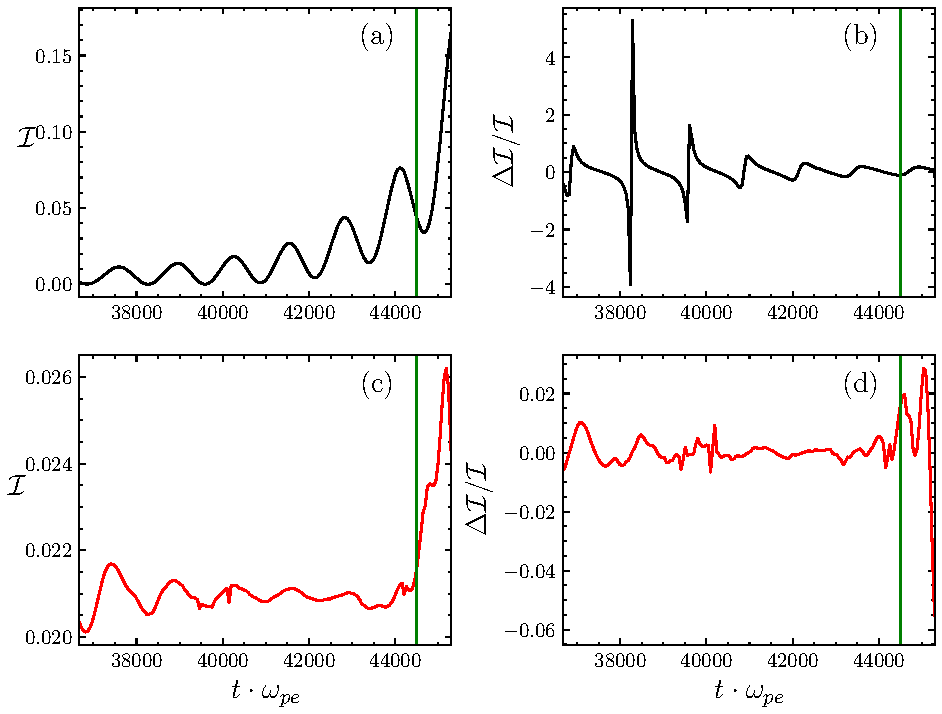
\includegraphics[scale=0.5]{img/adiaI.pdf}
    \caption{Time variation and  relative change of $\mathcal{I}$ for the test particle in the static (the black lines) and  real-time resonance  frames (the red lines). The green vertical line denotes the critical time when the conservation of $\mathcal{I}$ is violated.
     %and (d) shows the relative change of $\mathcal{I}$ with time.(a) and (b) 
    }
    \label{fig.I}
\end{figure}
To quantitatively show the adiabaticity, we numerically calculate the area of the phase loop and show its time variation 
%in Fig. \ref{fig.I}(a) and \ref{fig.I}(c). We also show 
and the relative error of the adiabatic invariant $\mathcal{I}(t)$ in Fig. \ref{fig.I}.
%figure \ref{fig.I} (b) and (d).
Unlike the static frame, the variation of $\mathcal{I}$ is less than $2\%$ in the reference frame following with the resonance, as seen in Fig. \ref{fig.I}(d). 
The adiabatic invariant $\mathcal{I}$ and the validity of the adiabaticity are shown to be conserved. 
The variation becomes large until the particle approaches the equator, where the wave amplitude is small, and the particle can be released from the wave potential well. 
The releasing of trapped particle, which is reported in the particle in cell (PIC) simulation \cite{tao_trap-release-amplify_2021}, could be a potential reason for the violation of the adiabatic motion.
% \begin{figure}
%     \centering
%     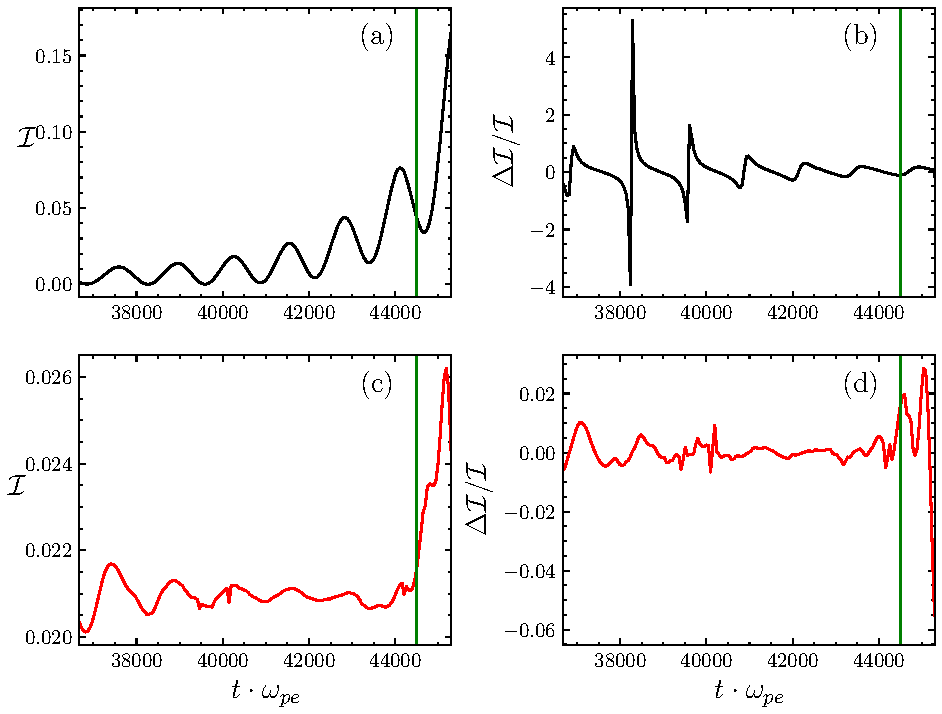
\includegraphics[scale=0.8]{img/adiaI.pdf}
%     \caption{The calculated $\mathcal{I}$ of a given particle in the static frame of reference and the compensated resonance reference.
%     }
%     \label{fig.I}
% \end{figure}

% \begin{figure}
%     \centering
%     \includegraphics[scale=0.8]{img/adiaIR.pdf}
%     \caption{The relative increment of $\mathcal{I}$ for a given particle in the static frame of reference and the compensated resonance reference. 
%     \label{fig.Ierr}
%     }
% \end{figure}
% %\if{1}
% \section{The adiabatic approximation}
%solve current integral and obtain the chirping law
%Nevertheless, harnessing 
With the adiabatic approximation, we can greatly reduce the description of the trapped particle distribution and the energetic particle current.
%In our previous studies, we obtain 
The nonlinear energetic particle current $j_p$ is obtained from the velocity integral of the perturbed distribution function 
\cite{zheng2024}
\begin{equation}\label{eq.ep_current}
    \begin{aligned}
j_p(s_i,t) & = -\frac{1}{ 4 \pi } \frac{\omega_{h0}^2k_i}{e}\iiint \sqrt{2m_e\omega_{ce}(s)(\mathcal{J}+\Omega+\Pi_i)} 
 \\
 &\times f(\xi,\Omega,\mathcal{J};s_i(t),t)e^{\imath \xi} \rm d \xi \rm d \Omega \rm d \mathcal{J}~.
    \end{aligned}
\end{equation}
%The current dominates the nonlinear behavior of the chorus chirping process, and under certain condition, we can simplify the phase space integral and show qualitatively how does the current evolves.
At the nonlinear stage, the distribution function of the trapped electrons forms a hole in phase space.
% and we consider its  $\Delta f$, .
Since the equilibrium distribution does not contribute to the current, the nonlinear current is directly determined by 
the deviation from the unperturbed distribution, i.e., the depth of the hole,
$\Delta f$.
The depth of the hole can be written as the function of the adiabatic invariant, i.e., $\Delta f(s_i,\mathcal{J},\mathcal{I},\xi,t)$.
Now we replace $f$ by $\Delta f$ in the current integral in Eq. (\ref{eq.ep_current}) and write  the integral as
\begin{equation}
\begin{aligned}
    j_p(s_i,t) & \approx - \int\mathrm{d} \mathcal{J} \sqrt{2 \omega_{ce} (\mathcal{J} + \Pi_i(t))}
    \\
    &\times \int_0^{\mathcal{I}_{\mathrm{s p x}}}  \mathrm{d}\mathcal{I}  \oint \mathrm{d}\psi  \Delta f(s_i,\mathcal{J},\mathcal{I},\xi,t)e^{\imath \xi}  ~.
\end{aligned}
\end{equation}
Note that $\Omega$ in the square root has been  neglected since $\Omega \simeq 0$.
The differential area element $\mathrm{d}\xi\mathrm{d}\Omega$ is changed to $\mathrm{d}\mathcal{I}\mathrm{d}\psi$, where $\psi$ is the angle variable of $\mathcal{I}$.
From the Jacobi of the differential element, the integral over $\psi$ is
\begin{equation}
    \begin{aligned}
      \oint f \mathrm{d}\psi & = \oint f \frac{\mathrm{d}\Omega}{\mathrm{d}\mathcal{I}}\mathrm{d}\xi = \frac{\partial H}{\partial \mathcal{I}} \oint f \frac{\mathrm{d}\Omega}{\mathrm{d} H}\mathrm{d}\xi = \dot{\psi}\oint \frac{f}{\Omega} \mathrm{d}\xi
      \\
      &\equiv 2 \pi \langle f \rangle,
    \end{aligned}
\end{equation}
where $\langle\cdots\rangle$ denotes the bounce average, following the definition in Ref. \cite{berk1999}.
Thus the current integral becomes
\begin{equation}\label{eq.adiabatic_current}
\begin{aligned}
    j_p(s_i,t)  &\approx -  {2\pi} \int\mathrm{d} \mathcal{J}  \sqrt{2\omega_{ce} (\mathcal{J} + \Pi_i(t))} \\
    & \times 
    \int_0^{\mathcal{I}_{\mathrm{s p x}}}\mathrm{d}\mathcal{I}  \langle \Delta f(s_i,\mathcal{J},\mathcal{I},\xi,t)e^{\imath \xi} \rangle  ~.
\end{aligned}
\end{equation}
%For the adiabatic regime, the characteristic scales should vary considerably slowly compared to the wave trapping scale.
%There exists a small scale $\epsilon$ satisfies \cite{berk1999}
%\begin{equation}
%    \epsilon \equiv \mathrm{max}\left(\ddot{\omega}/\omega_b^3, \dot{\omega}/\omega_b^2, \omega_b/\omega \right) \ll 1~,
%\end{equation}
%Here, $\omega$ is the frequency deviation from the resonance center in our context.
%For the chorus wave field, the frequency, and other quantities change slowly in one bounce period, satisfying the first and the second inequalities. The last term requires the frequency chirped a notable distance, i.e., the nonlinear stage, where the hole has been separated from the equilibrium.
Note that $\Delta f$ can be expanded in powers of $\epsilon$, a small parameter describing the change of parameters during the bounce motion
%Following  the method in Ref. \cite{berk1999}, 
and the bounce averages in Eq.~(\ref{eq.adiabatic_current}) are 
 \cite{berk1999} 
\begin{equation}
    \begin{aligned}
    \langle\Delta f \sin \xi \rangle &\simeq \alpha \Delta f_0 ~, \\ 
    \langle \Delta f \cos \xi \rangle &\simeq  \Delta f_0 \langle \cos \xi \rangle ~.
    \end{aligned}
\end{equation}
%approximation 2, I is constant over trapped region
We further assume that $\Delta f_0$ is independent of $\mathcal{I}$, which implies that the depth of the hole is flat within the enclosed hole area, i.e., the water bag approximation \cite{omura_theory_2008,hezaveh2021}. 
Therefore, the integral over $\mathcal{I}$ only depend on the $\mathcal{I}_\mathrm{spx}$ which is the 
 adiabatic invariant on the separatrix. 
According to Eq. (\ref{eq.def_I}), we have
\begin{equation}
    \int^{\mathcal{I}_\mathrm{s p x}}_0 \mathrm{d}\mathcal{I} = \mathcal{I}_\mathrm{s p x} \equiv {1\over2\pi} \oint_\mathrm{s p x} \Omega (\xi) \mathrm{d} \xi~,
\end{equation}
where the boundary of the trapped particle phase space hole can be analytically given as
\begin{equation}
    \Omega(\xi) = \pm \frac{\omega_b}{k^2} \sqrt{2 (e_\mathrm{spx}-\cos \xi - \alpha \xi)}~,
\end{equation}
and $e_\mathrm{spx}$ denotes the Hamiltonian on the separatrix.
%, cf. ref. \cite{zheng2023b}.
%Now we define two functions of $\alpha$
Then the current integral becomes  
\begin{equation}\label{eq.adi_J}
    \begin{aligned}
    j_p(s_i,t) & \approx \frac{\sqrt{2} \omega_b}{k^2}  \left(m_\mathrm{s p x}+\imath ~ n_\mathrm{s p x}\right) \\
    & \times  \int \mathrm{d} \mathcal{J} \sqrt{ \omega_{c e}(\mathcal{J}+\Pi_i(t))} \Delta f(\mathcal{J},s_i,t) ~,
    \end{aligned}
\end{equation}
where
\begin{equation}\label{eq.function}
    \begin{aligned}
        m_\mathrm{spx}(\alpha) & = \oint_\mathrm{s p x} \mathrm{d} \xi \cos \xi \sqrt{e_\mathrm{s p x}-\cos \xi-\alpha \xi}, 
        \\
        n_\mathrm{spx}(\alpha) &  = \alpha \oint_\mathrm{s p x} \mathrm{d} \xi \sqrt{e_\mathrm{s p x}-\cos \xi-\alpha \xi}.
    \end{aligned}
\end{equation}
%the nonlinaer currnet and the chirping rate ...
%differnece with omura 
%process approxiamtion strict follows adiabatic approximation
%why the hole is oblique
%alpha value should small to validate approximation
%figure
\begin{figure}
    \centering
    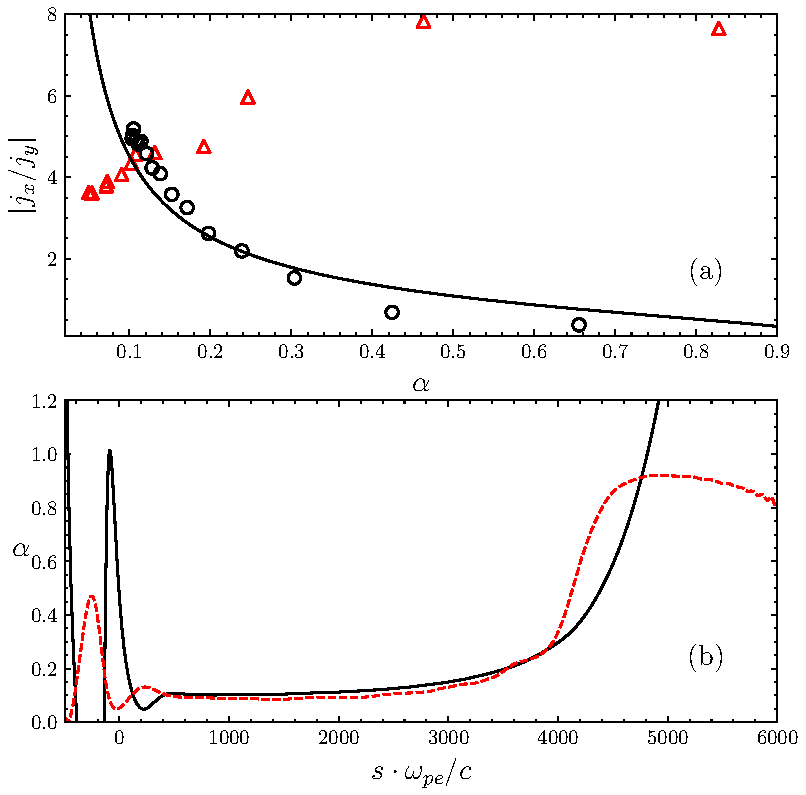
\includegraphics[scale=0.5]{img/alpha.pdf}
    \caption{(a) Current ratio versus the inhomogeneous parameter $\alpha$. The scattered points are obtained at difference spatial locations from the simulation, the triangles are obtained from near the equator region while circus are obtained from the downstream region. 
    The solid curve is the results from adiabatic approximation Eq. (\ref{eq.adia_relation}). 
    (b) Snapshot  of the parameter $\alpha$ at $t = 850$ obtained  from the definition in Eq. (\ref{eq.alpnew}) (black solid line) and  from adiabatic relation (red dashed line).
    }
    \label{fig.adiabatic}
\end{figure}


%A $\delta f$ Vlasov equation coupled with a wave envelope equation are given and self-consistently describes the wave-particle interactions.
%Here, we recall the Vlasov equation for $\delta f(s_i,\vartheta,\mathcal{J},\xi,\Omega)$ 
%\begin{equation}\label{eq.vlasov}
%    \frac{\partial \delta f}{\partial t} + \frac{d s_{i}}{d t} \frac{\partial \delta f}{\partial s_{i}} + \frac{d\mathcal{J}}{dt}\frac{\partial \delta f}{\partial \mathcal{J}} + \frac{\partial \delta f}{\partial \xi}\frac{d \xi}{dt} + \frac{\partial \delta f}{\partial \Omega}\frac{d \Omega}{d t}  = \frac{\partial f_0}{\partial \Omega}\frac{\partial \delta K}{\partial \xi}~,
%\end{equation}
%where $\delta K$ = 
%
%The constant for each cell is determined by the initial choice of $\mathcal{J}$, which give the entire information of the dynamics on the slowly varying scale along the magnetic field line.
%The equations for the fast varying compontens
%\begin{equation}\label{eq.odes2}
%    \begin{aligned}
%    \frac{\mathrm{d}\Omega}{\mathrm{d}t} &= \frac{\omega_b^2}{k_i^2}\left(\sin \xi - \alpha \right)~,
%    \\
%    \frac{\mathrm{d}\xi}{\mathrm{d}t} &= {k_{i}^{2}\Omega}+ \frac{\omega_{ce} }{\sqrt{2\omega_{ce}(\mathcal{J}+\Omega+\Pi_i)}}\frac{e |a|}{c}\cos \xi ~.
%    \end{aligned}
%\end{equation}
%and 
%\begin{equation}\label{eq.alp1}
%   \alpha \simeq \frac{k_l}{\omega_b^2}\left(\mathcal{J}-\frac{\Pi_i}{2}\right) \frac{\partial \omega_{c e}}{\partial s}
%\end{equation}
%
%The wave equation 
%\begin{equation}\label{eq.full}
%    \frac{\partial a}{\partial t} +v_g \frac{\partial a}{\partial s_i} =\frac{-\imath 2\pi v_g}{c k_i } j_p~,
%\end{equation}
%for reference.
%The energetic particle current $j_p$ is
%\begin{equation}\label{eq.ep_current}
%j_p(s_i,t) = -\frac{1}{ 4 \pi } \frac{\omega_{h0}^2k_i}{e}\iiint \sqrt{2m_e\omega_{ce}(s)(\mathcal{J}+\Omega+\Pi_i)} \times f(\xi,\Omega,\mathcal{J};s_i(t),t)e^{\imath \xi} \rm d \xi \rm d \Omega \rm d \mathcal{J}~,
%\end{equation}
The temporospatial evolution of the nonlinear current only depends on the integral over the slowly varying scale $\mathcal{J}$, and an inhomogeneity parameter $\alpha$, defined in Eq. (\ref{eq.alpnew}). 
The $\mathcal{J}$ integral can be calculated further with the adiabatic motion of the trapped particle along the magnetic field line \cite{summers2012}, while the integrals $m_\mathrm{spx}$ and $n_\mathrm{spx}$ can be numerical integrated from Eq. (\ref{eq.function}).
%Since the phase space hole is aligned with the slowly varying wave packet, the hole depth $\Delta f$ also contributes to a complex phase $\delta \phi(s,t)$, which is the phase of the slowly varying wave packet $\delta \phi \equiv \arg(a)$.
Note that, our Vlasov simulation is performed with Hamiltonian Eq. (\ref{eq.H_lab}), thus the phase of the current $j_p$ in the Vlasov simulation also differs $\delta \phi$ with the current relation in Eq. (\ref{eq.adi_J}).
To compared and verify our adiabatic theory, we should also translate this addition phase, i.e., $j^\prime_{p} = j_p \cdot e^{-\imath \delta \phi}$, where $j_p$ is the current from Vlasov equation. 
From Eqs. (\ref{eq.adi_J}) and (\ref{eq.function}), we can find that the ratio of the imaginary and real component of $j^\prime_{p}$ is a function of $\alpha$, 
\begin{equation}\label{eq.adia_relation}
\frac{j_x}{j_y} = \frac{\mathrm{real}(j^\prime_p)}{\mathrm{imag}(j^\prime_p)} = \frac{m_\mathrm{spx}(\alpha)}{n_\mathrm{spx}(\alpha)}
\end{equation}

By numerically solve the integral in Eq. (\ref{eq.function}), we obtain an explicit relation of current ration with respect to $\alpha$ shown in Fig. \ref{fig.adiabatic}(a). 
Meanwhile, to verify the validity of the relation, we select various spatial locations at $t=850$ from the Vlasov simulation \cite{zheng2023b,zheng2024}, calculate the $\alpha$ from definition in Eq. (\ref{eq.alpnew}), and get the corresponding current ratio.
It is shown that the value obtained in our simulation result well agree with the adiabatic predictions in propagation region of the chorus wave (black circles).
Conversely, the above relation can be applied as an alternative way for evaluating the inhomogeneous parameter $\alpha$ from the energetic particle current, which might be more accurate if the current can be measured somehow.
It is meaningful since the inhomogeneous parameter $\alpha$ is of importance to study the wave-particle interaction and chirping behavior \cite{tao_theoretical_2020,omura2008}.
%The relation provides an alternative way   ,  
%Unlike to the calulating $\alpha$ from the definition, we only need to know the current 

Nevertheless, near the equator region, where the chorus is triggered, (red triangles), the adiabatic approximation is no longer valid.
Similar conclusion can be drawn from the spatial distribution of $\alpha$ calculated from definition in Eq. (\ref{eq.alpnew}) and the adiabatic current relation, as shown in Fig. \ref{fig.adiabatic}(b). 
The evolution of $\alpha$ indicates a rapid variation of the phase space near the equator, which is related to the generation of the nonlinear chorus wave.
The results of nonadiabtic regime also agree with the previous PIC simulations \cite{tao2017a,tao2017b}.
